\documentclass[a4paper]{article}

\usepackage[utf8x]{inputenc}
\usepackage[british,UKenglish]{babel}
\usepackage{amsmath}
%\usepackage{titlesec}
\usepackage{color}
\usepackage{graphicx}
\usepackage{fancyref}
\usepackage{hyperref}
\usepackage{float}
\usepackage{scrextend}
\usepackage{setspace}
\usepackage{xargs}
\usepackage{multicol}
\usepackage{nameref}
\usepackage[pdftex,dvipsnames]{xcolor}
\usepackage{sectsty}
\usepackage{multicol}
\usepackage{multirow}
\usepackage[procnames]{listings}
\usepackage{appendix}

\newcommand\tab[1][1cm]{\hspace*{#1}}
\hypersetup{colorlinks=true, linkcolor=black}
\interfootnotelinepenalty=10000
%\titleformat*{\subsubsection}{\large\bfseries}
\subsubsectionfont{\large}
\subsectionfont{\Large}
\sectionfont{\LARGE}
\definecolor{cleanOrange}{HTML}{D14D00}
\definecolor{cleanYellow}{HTML}{FFFF99}
\definecolor{cleanBlue}{HTML}{3d0099}
%\newcommand{\cleancode}[1]{\begin{addmargin}[3em]{3em}\fcolorbox{cleanOrange}{cleanYellow}{\texttt{\textcolor{cleanOrange}{#1}}}\end{addmargin}}
\newcommand{\cleancode}[1]{\begin{addmargin}[3em]{3em}\texttt{\textcolor{cleanOrange}{#1}}\end{addmargin}}
\newcommand{\cleanstyle}[1]{\text{\textcolor{cleanOrange}{\texttt{#1}}}}


\usepackage[colorinlistoftodos,prependcaption,textsize=footnotesize]{todonotes}
\newcommandx{\commred}[2][1=]{\textcolor{Red}
{\todo[linecolor=red,backgroundcolor=red!25,bordercolor=red,#1]{#2}}}
\newcommandx{\commblue}[2][1=]{\textcolor{Blue}
{\todo[linecolor=blue,backgroundcolor=blue!25,bordercolor=blue,#1]{#2}}}
\newcommandx{\commgreen}[2][1=]{\textcolor{OliveGreen}{\todo[linecolor=OliveGreen,backgroundcolor=OliveGreen!25,bordercolor=OliveGreen,#1]{#2}}}
\newcommandx{\commpurp}[2][1=]{\textcolor{Plum}{\todo[linecolor=Plum,backgroundcolor=Plum!25,bordercolor=Plum,#1]{#2}}}

\def\code#1{{\tt #1}}

\def\note#1{\noindent{\bf [Note: #1]}}
% "define" Scala
\usepackage[T1]{fontenc}  
\usepackage[scaled=0.82]{beramono}  
\usepackage{microtype} 

\sbox0{\small\ttfamily A}
\edef\mybasewidth{\the\wd0 }

\lstdefinelanguage{scala}{
  morekeywords={abstract,case,catch,class,def,%
    do,else,extends,false,final,finally,%
    for,if,implicit,import,match,mixin,%
    new,null,object,override,package,%
    private,protected,requires,return,sealed,%
    super,this,throw,trait,true,try,%
    type,val,var,while,with,yield},
  sensitive=true,
  morecomment=[l]{//},
  morecomment=[n]{/*}{*/},
  morestring=[b]",
  morestring=[b]',
  morestring=[b]"""
}

\usepackage{color}
\definecolor{dkgreen}{rgb}{0,0.6,0}
\definecolor{gray}{rgb}{0.5,0.5,0.5}
\definecolor{mauve}{rgb}{0.58,0,0.82}

% Default settings for code listings
\lstset{frame=tb,
  language=scala,
  aboveskip=3mm,
  belowskip=3mm,
  showstringspaces=false,
  columns=fixed, % basewidth=\mybasewidth,
  basicstyle={\small\ttfamily},
  numbers=none,
  numberstyle=\footnotesize\color{gray},
  % identifierstyle=\color{red},
  keywordstyle=\color{blue},
  commentstyle=\color{dkgreen},
  stringstyle=\color{mauve},
  frame=single,
  breaklines=true,
  breakatwhitespace=true,
  procnamekeys={def, val, var, class, trait, object, extends},
  procnamestyle=\ttfamily\color{red},
  tabsize=2
}

\lstnewenvironment{scala}[1][]
{\lstset{language=scala,#1}}
{}
\lstnewenvironment{cpp}[1][]
{\lstset{language=C++,#1}}
{}
\lstnewenvironment{bash}[1][]
{\lstset{language=bash,#1}}
{}
\lstnewenvironment{verilog}[1][]
{\lstset{language=verilog,#1}}
{}



\lstset{frame=, basicstyle={\footnotesize\ttfamily}}



\graphicspath{ {images/} }

%-----------------------------------------BEGIN DOC----------------------------------------

\begin{document}

\title{{\Huge ercesiMIPS Lab Manual{\large\linebreak\\}}{\Large A guide to Pipeline CPU with MIPS 32 ISA Supports\linebreak\linebreak}
\linebreak{\Large[\nameref{c}]}
\linebreak{\small click on it\linebreak}}
\author{\\Authors: Jianfeng An, Meng Zhang \& Danghui Wang\\\\
CS 11007 Computer Organization and Architecture\\
(May, 2017)\\\\
Northwestern Polytechnical University, China\\
Faculty of Computer Science\\
ERCESI}
\date{21 May 2017}
\maketitle
\newpage

%-----------------------------------------ABSTRACT-------------------------------------

{\large\bf{"SWEET JEZUS WHY!?"\\}}
\begin{addmargin}[2em]{2em}{\setstretch{0.6}{\small\textit{If you're reading this, chances are that either your arms are suffering from anemia in waiting for the TA's to finish helping the 20 people in the room, or you're trying to design in Chisel without any TA's whatsoever, and you just wanna end it all. Fret not! This document serves as a specification for basic explanations of single cyclic MIPS CPU with 7-11 instructions supporting, also a helpful links and forbidden deigning secrets whose names none dare speak.}}}
\end{addmargin}
\tableofcontents\label{c}
\newpage

%------------------------------------------TEXT--------------------------------------------

%----------------------------------------OVERVIEW-----------------------------------------

\section{Overview} \label{overview}%------------------------------
The structure of Multi cyclic MIPS CPU has been introduced in CS 11007 class lecture.
\begin{itemize}
	\item{\textbf{MIPS 32 ISA} includes \emph{sub, add, ori, lw, sw, beq, j}, or adding \emph{addi, and, andi, or, slt} for better programming experience in assembly. All these instructions can be supported without exception detecting (overflow detecting)}
    \item{\textbf{These instructions work in different multi cycles.} A very basic concept adopted here is that the multi cycles are controlled by FSM (Finite State Machine).}
    \item{\textbf{Consisted of Data Path, Control Unit and Memory Unit.} To illustrate the typical systematic idea of computer, we recommend you design your first CPU with two separated modules, CPath and DPath, in such coding style, both blocks can also be easily verified separately. Additionally, if more complement MIPS ISA is chosen, this structure will be high efficient to be extended.}
    \item{\textbf{Chisel3 is also recommended.}}
\end{itemize}

%-----------------------------------------Specification-------------------------------------------

\newpage
\section{Specification} \label{Specification}%------------------------------
A typical multi cyclic CPU core can also be consisted of Control Unit and Data Path unit. Although there is no big picture for a whole multi cyclic CPU, in our lecture 12, Fig. \ref{fig:multiblock} still can be figured out by composing several slides. 
\begin{figure}[ht]
 \centering
 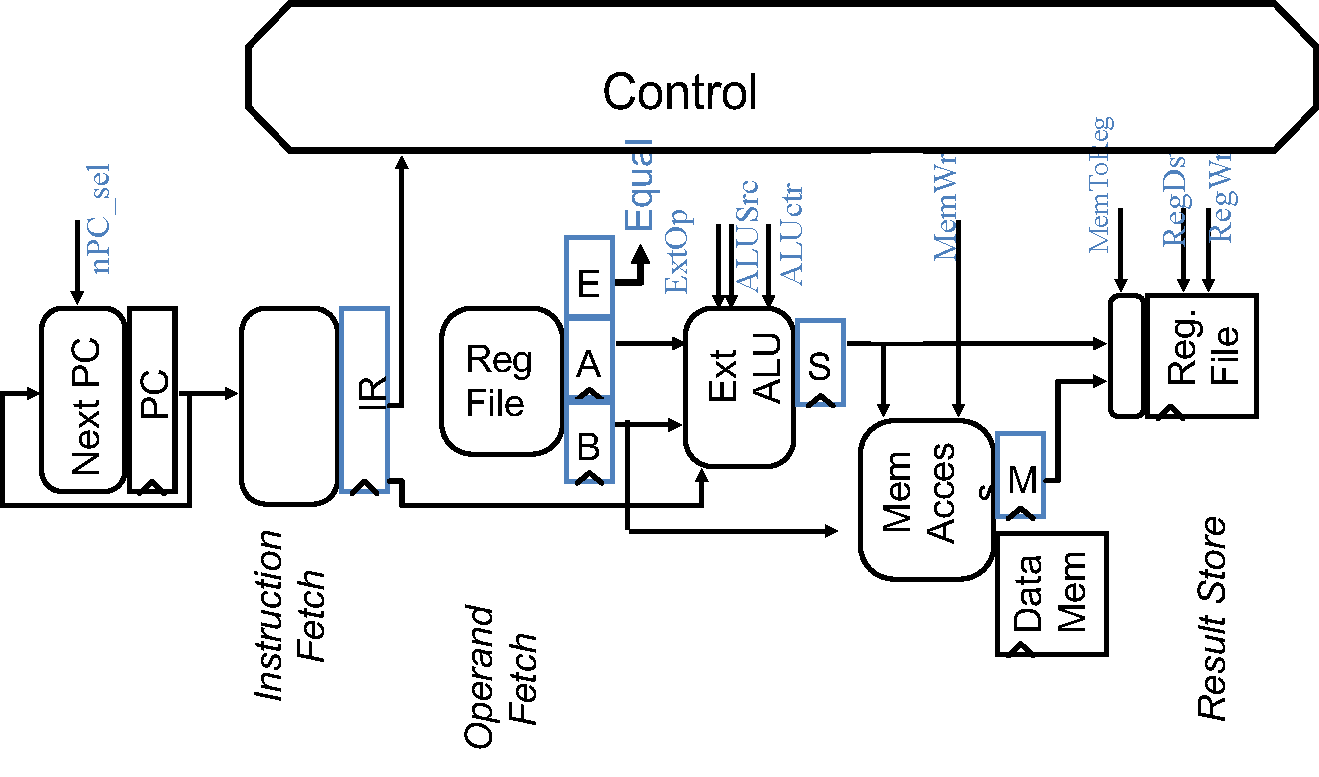
\includegraphics[height=5cm]{images/l2sys.pdf}
 \caption{Multi Cyclic CPU Block Diagram}
 \label{fig:multiblock}
\end{figure}

\textbf{Two Module classes are still recommended, Control Unit and Data Path Unit respectively}, as shown in following Fig. \ref{fig:modules}. To simply the design, Harvard structure is still adopted in multi cyclic CPU lab, a MIPS adaptive memory model (Princeton Structure) is mandatory in further pipeline structure.  
\begin{figure}[ht]
 \centering
 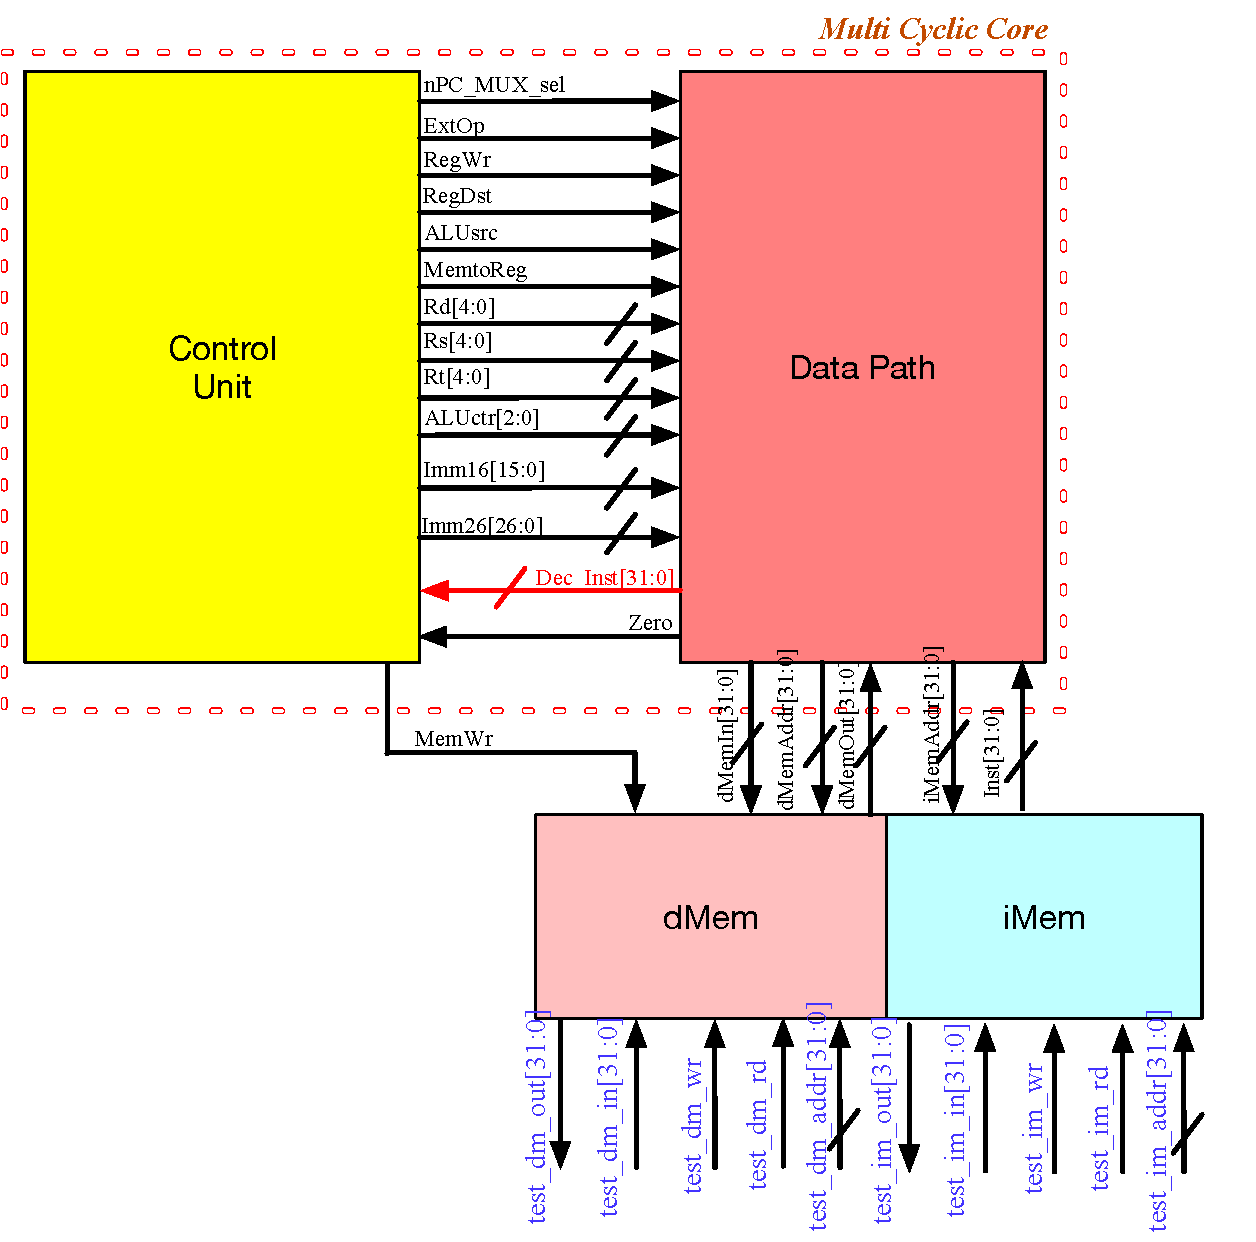
\includegraphics[height=7cm]{images/l2modules.pdf}
 \caption{Multi Cyclic CPU Block Diagram}
 \label{fig:modules}
\end{figure}
In Fig. \ref{fig:modules}, a \textbf{red} marked signal bus, \code{Dec\_Inst[31:0]}, is recommend as a \code{IR} output for FSM Decode state. Almost all signals can be renamed by your self except those evaluation required singles specified in Section \ref{sub:signal}.
%---------------------------------------Chisel 3------------------------------------------

\newpage
\section{Chisel3 101} \label{chisel3}%------------------------------
\subsection{FSM in Chisel}\label{sub:FSM}
TBD

%-------------------------------Evalu Req------------------------------------------

\newpage
\section{Evaluation Requirement} \label{sec:Functions}%------------------------------
We (or TAs) will check and evaluate your design with a pre-coded test program, in which a pseudo-random instruction queue will be feed into you instruction memory and data memory. To ensure this test works correctly, the test signal interfaces name \textbf{MUST} meets the requirements shown in Table \ref{tab:signaldef}.
\subsection{Test Procedure}\label{sub:TestProc}
As Operation System is still not available for this stage, the program and initial data are feed into Instruction Memory and Data Memory from the Tester program respectively. By utilizing \code{ori} instruction, the Tester program provides an alternative data memory initialization, \code{\$t = \$zero | imm16} (\code{ori, rt, \$zero Imm16}). In which, \code{\$t} stores the result of \textit{or} operation (immediate "or" zero register), i.e. the immediate is loaded into register file by \code{ori} instruction.

\begin{figure}[ht]
 \centering
 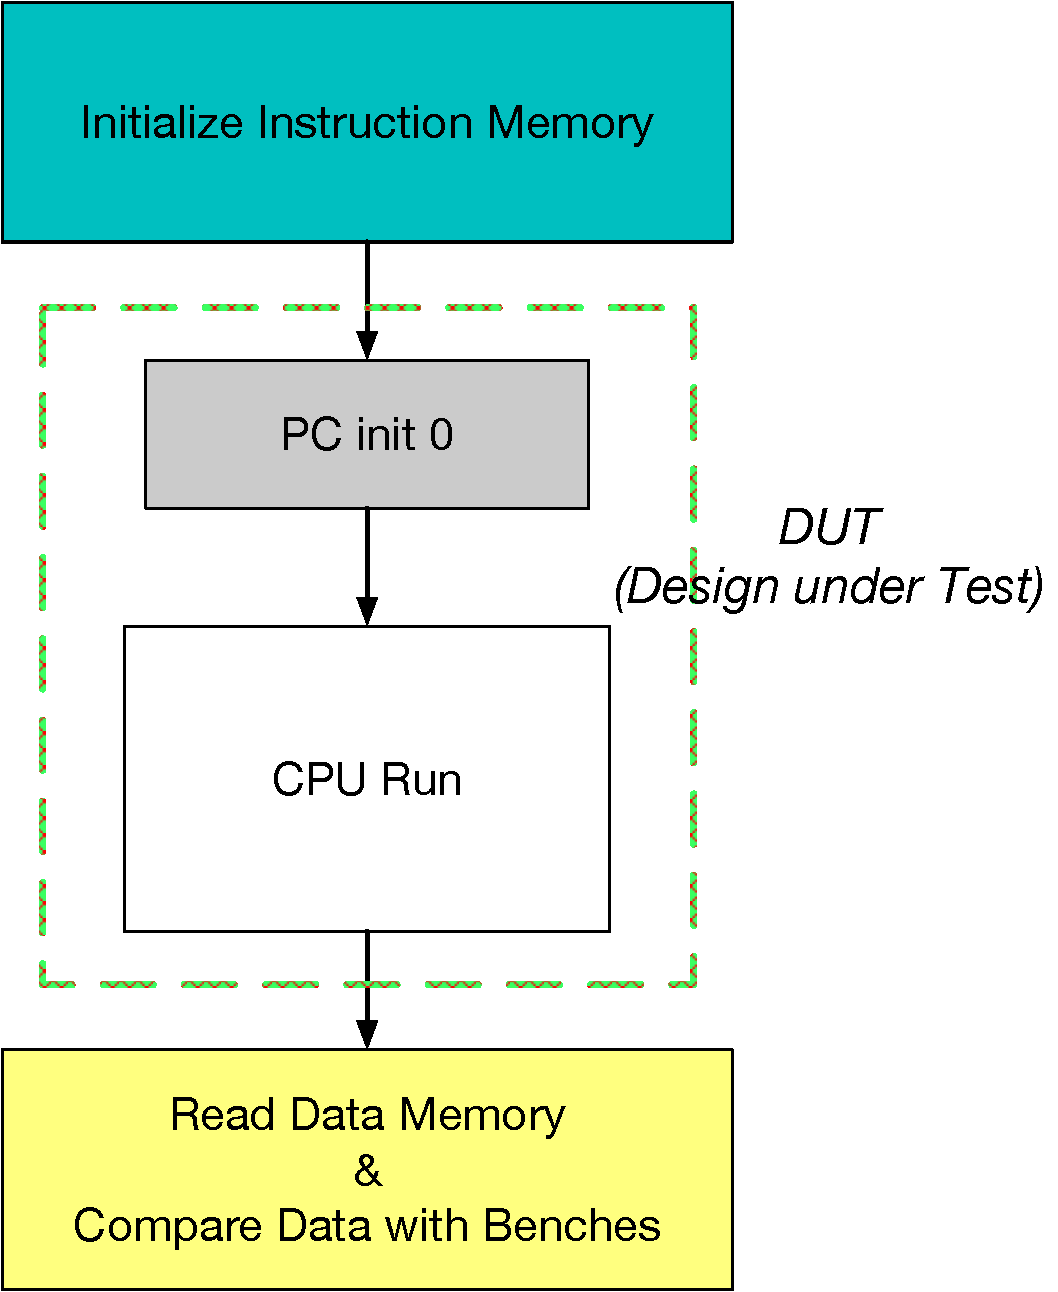
\includegraphics[height=7cm]{images/l1TestProc.pdf}
 \caption{Test Procedure}
 \label{fig:testproc}
\end{figure}

Fig. \ref{fig:testproc} shows the whole test procedure. In which, the designed CPU is denoted by DUT (Design under Test), the instruction is feed into Imem at the initialization stage, and the data about how program running is collected at the end.

\subsection{Signals for Test mode}\label{sub:signal}

\begin{figure}[ht]
	\centering
	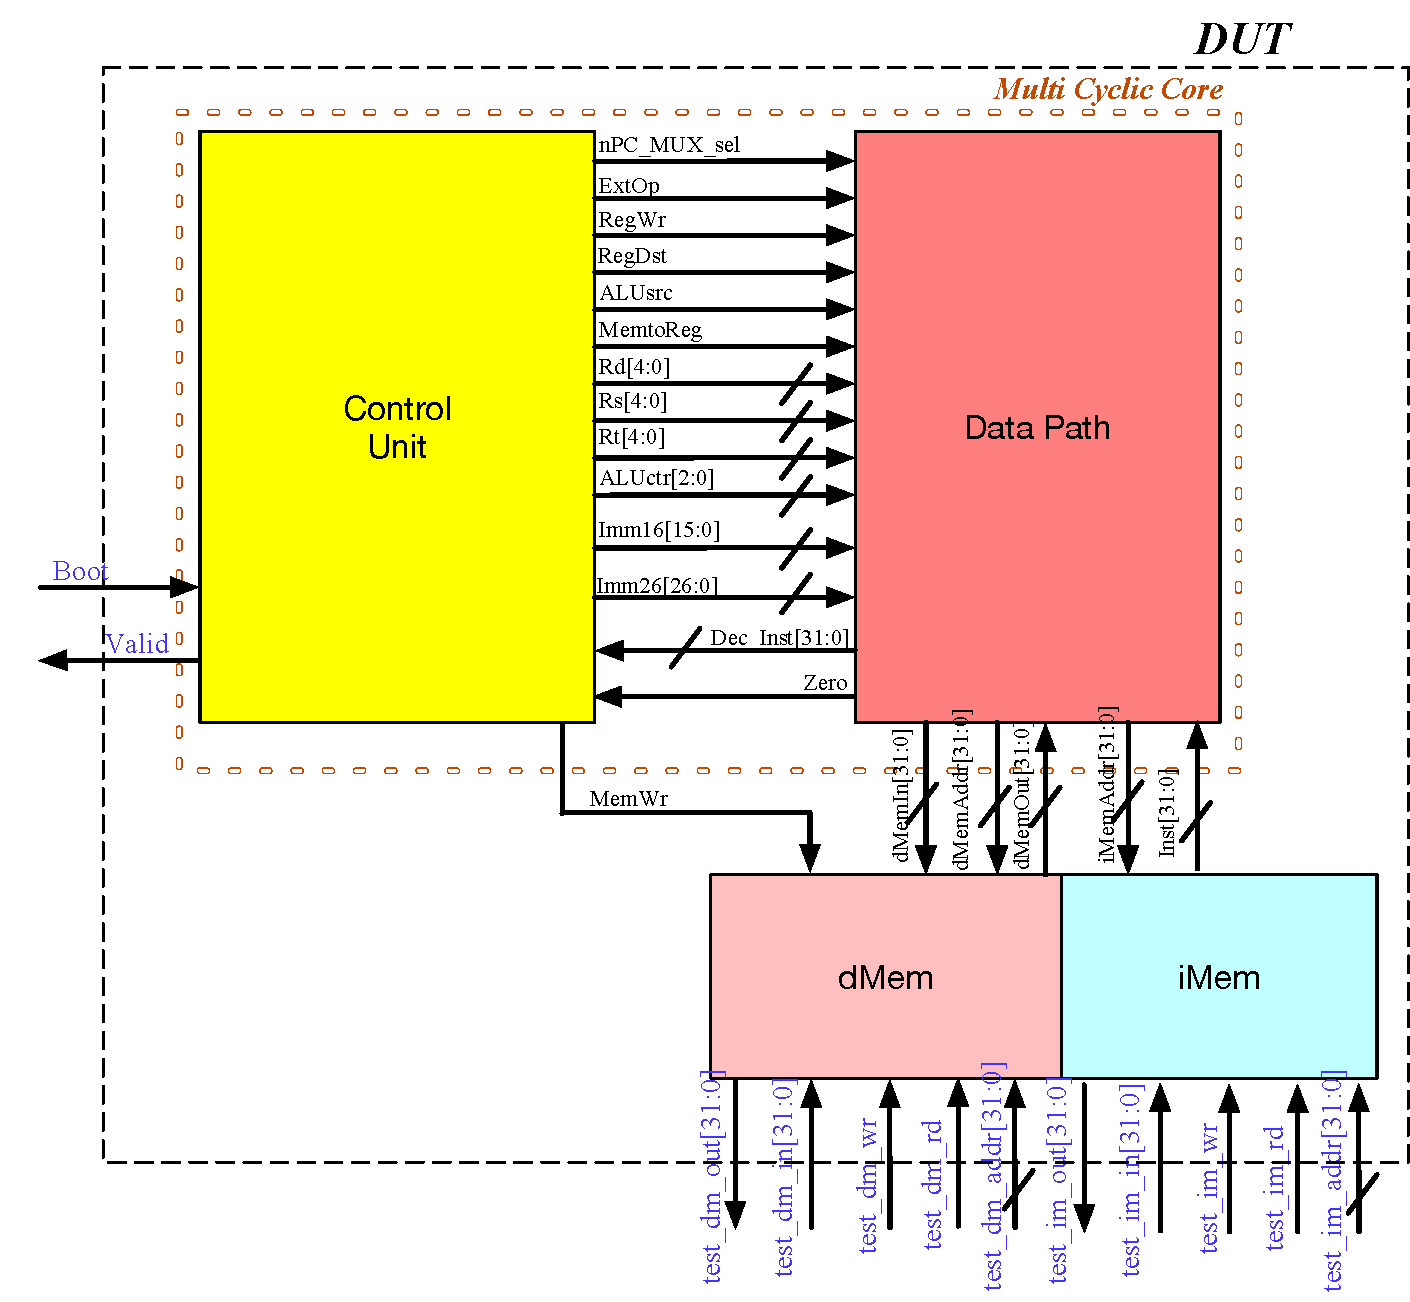
\includegraphics[height=9cm]{images/l2ModulesTest.pdf}
	\caption{Top Block Diagram for Test Mode}
	\label{fig:moduletest}
\end{figure}
%\url{}
The recommended Top block structure is shown in Fig. \ref{fig:moduletest}, which the blue marked interfaces are connected with testbench. So please define these interfaces in your top module as exactly the same as Table \ref{tab:signaldef} shown.

\begin{table}[htp]
\caption{Signals Definition for Test Mode}\label{tab:signaldef}
\begin{center}
	\begin{tabular}{|l|l|l|p{6cm}|}
	\hline
	\textbf{Signal Name} & \textbf{Direction} & \textbf{Width} & \textbf{Function}\\ \hline \hline
	boot			& Input 	& 1-bit	& Trigger the boot test mode, 
									  set to 0 in CPU regular process mode\\ \hline
	test\_im\_wr 	& Input	& 1-bit	& Instruction memory write enable in test mode,set to 0 in 	
								  CPU regular process mode. In test mode, it will be set to 1 when if writing instructions to imem, otherwise it is set to 0.\\ \hline
	test\_im\_re 	& Input & 1-bit & Instruction memory read enable in test mode,set to 0 in 	
								  CPU regular process mode. In test mode, it will be set to 1 when if reading instructions out, otherwise it is set to 0. \\ \hline
	test\_im\_addr 	& Input & 32-bit& Instruction memory address\\ \hline
	test\_im\_in 	& Input & 32-bit& Instruction memory data input for test mode. \\ \hline
	test\_im\_out 	& Output& 32-bit& Instruction memory data output for test mode. \\ \hline
	test\_dm\_wr 	& Input	& 1-bit	& Data memory write enable in test mode,set to 0 in 	
								  CPU regular process mode. In test mode, it will be set to 1 when if writing data to dmem, otherwise it is set to 0.\\ \hline
	test\_dm\_re 	& Input & 1-bit & Data memory read enable in test mode,set to 0 in 	
								  CPU regular process mode. In test mode, it will be set to 1 when if reading data out, otherwise it is set to 0.\\ \hline
	test\_dm\_addr 	& Input & 32-bit& Data memory address\\ \hline
	test\_dm\_in 	& Input & 32-bit& Data memory input for test mode. \\ \hline
	test\_dm\_out 	& Output& 32-bit& Data memory output for test mode. \\ \hline
	valid			& Output& 1-bit & If CPU stopped or any exception happens, valid signal is set to 0.\\ 
	\hline
	\end{tabular}
\end{center}
\end{table}

Additionally, a \code{valid} signal is highly recommended. It can be monitored to find whether CPU works correctly. As shown in Table \ref{tab:signaldef}, \code{valid} will be set to 0, if the fetched instruction is not defined in our 7-Inst ISA (e.g. \code{0xFFFFFFFF}), which is to tell test the CPU is working in exception.

\subsection{Basic Logic for Test}\label{sub:testlogic}
Please add the test logic into your top module as shown in Table \ref{tab:logic}.\\
The \code{Top} Module is presented below, please \textbf{DO NOT} change any code of Top module:
\begin{scala}
package MultiCycle

import chisel3._
import chisel3.iotesters.Driver
//import utils.ercesiMIPSRunner
class TopIO extends Bundle() {
	val boot = Input(Bool()) 
// imem and dmem interface for Tests
	val test_im_wr		= Input(Bool())
	val test_im_rd 		= Input(Bool())
	val test_im_addr 	= Input(UInt(32.W))
	val test_im_in 		= Input(UInt(32.W))
	val test_im_out 	= Output(UInt(32.W))

	val test_dm_wr		= Input(Bool())
	val test_dm_rd 		= Input(Bool())
	val test_dm_addr 	= Input(UInt(32.W))
	val test_dm_in 		= Input(UInt(32.W))
	val test_dm_out 	= Output(UInt(32.W))

	val valid			= Output(Bool())
}

class Top extends Module() {
	val io 		= IO(new TopIO())//in chisel3, io must be wrapped in IO(...) 
	val cpath	= Module(new CtlPath())
	val dpath 	= Module(new DatPath())

	cpath.io.ctl <> dpath.io.ctl
	cpath.io.dat <> dpath.io.dat
	io.valid := cpath.io.valid
	cpath.io.boot := io.boot

	val imm = Mem(256, UInt(32.W))
	val dmm = Mem(1024, UInt(32.W))
	io.test_dm_out := 0.U
	io.test_im_out := 0.U
	cpath.io.Inst := 0.U
	when (io.boot && io.test_im_wr){
		imm(io.test_im_addr >> 2) := io.test_im_in
		cpath.io.Inst := 0.U
	 } 
	when (io.boot && io.test_dm_wr){
		dmm(io.test_dm_addr >> 2) := io.test_dm_in
		cpath.io.Inst := 0.U
	} 
	when (io.boot && io.test_im_rd){
		io.test_im_out := imm(io.test_im_addr >> 2)
		cpath.io.Inst := 0.U
	} 
	when (io.boot && io.test_dm_rd){
		io.test_dm_out := dmm(io.test_dm_addr >> 2)
		cpath.io.Inst := 0.U
	} 
	when (!io.boot){
		cpath.io.Inst := Mux(io.boot, 0.U, imm(dpath.io.imem_addr >> 2))
		dpath.io.dmem_datOut := dmm(dpath.io.dmem_addr >> 2)
		when (cpath.io.MemWr) {
			dmm(dpath.io.dmem_addr >> 2) := dpath.io.dmem_datIn
		}
	}
}
\end{scala}
\begin{table}[htp]
	\caption{Logic Operation in Test Mode}\label{tab:logic}
	\begin{center}
		\begin{tabular}{|l|c|c|}
		\hline
		\textbf{Operation}	& \textbf{Signal}	& \textbf{Boolean Logic} \\ \hline
		\multirow{5}{*}{Imem Write}& boot		& 1 \\ \cline{2-3}
							& test\_im\_wr 		& 1 \\ \cline{2-3}
							& test\_im\_rd 		& 0 \\ \cline{2-3}
							& test\_dm\_wr 		& 0 \\ \cline{2-3}
							& test\_dm\_rd 		& 0 \\ \hline
		\multirow{5}{*}{Dmem Write}& boot 		& 1 \\ \cline{2-3}
							& test\_im\_wr 		& 0 \\ \cline{2-3}
							& test\_im\_rd 		& 0 \\ \cline{2-3} 
							& test\_dm\_wr 		& 1 \\ \cline{2-3}
							& test\_dm\_rd 		& 0 \\ \hline
		\multirow{5}{*}{Imem Read}& boot 		& 1 \\ \cline{2-3}
							& test\_im\_wr 		& 0 \\ \cline{2-3}
							& test\_im\_rd 		& 1 \\ \cline{2-3} 
							& test\_dm\_wr 		& 0 \\ \cline{2-3}
							& test\_dm\_rd 		& 0 \\ \hline
		\multirow{5}{*}{Dmem Read}& boot 		& 1 \\ \cline{2-3}
							& test\_im\_wr 		& 0 \\ \cline{2-3}
							& test\_im\_rd 		& 0 \\ \cline{2-3} 
							& test\_dm\_wr 		& 0 \\ \cline{2-3}
							& test\_dm\_rd 		& 1 \\ \hline
		\end{tabular}
	\end{center}
\end{table}

\end{document}

